\documentclass[a4paper]{book}

\usepackage[hypcap=false]{caption}
\usepackage{enumitem}	% 定制enumerate标号
\usepackage{geometry}
\geometry{%
	left=2cm,%
	right=2cm,%
	top=2cm,%
	bottom=2cm,%
	bindingoffset=0cm
}
\usepackage{hyperref}
\hypersetup{
    colorlinks=true,            %链接颜色
    linkcolor=blue,             %内部链接
    filecolor=magenta,          %本地文档
    urlcolor=cyan,              %网址链接
    pdftitle={Overleaf Example},
    pdfpagemode=FullScreen,
}
\usepackage[none]{hyphenat}	% 阻止长单词分在两行
\usepackage{mathrsfs}	% 提供\mathscr字体
\usepackage[version=4]{mhchem}

\RequirePackage[many]{tcolorbox}
\tcbset{
    boxed title style={colback=magenta},
	breakable,
	enhanced,
	sharp corners,
	attach boxed title to top left={yshift=-\tcboxedtitleheight,  yshifttext=-.75\baselineskip},
	boxed title style={boxsep=1pt,sharp corners},
    fonttitle=\bfseries\sffamily,
}

\definecolor{skyblue}{rgb}{0.54, 0.81, 0.94}

\newtcolorbox[auto counter, number within=chapter, number format=\arabic]{exercise}[1][]{
    title={Exercise~\thetcbcounter},
    colframe=skyblue,
    colback=skyblue!12!white,
    boxed title style={colback=skyblue},
    overlay unbroken and first={
        \node[below right,font=\small,color=skyblue,text width=.8\linewidth]
        at (title.north east) {#1};
    }
}

\newtcolorbox[auto counter, number within=chapter, number format=\arabic]{solution}[1][]{
%    top=2ex,
%    boxrule=0pt,
%    leftrule=1.4pt,
    title={Solution~\thetcbcounter},
    colframe=teal!60!green,
    colback=green!12!white,
    boxed title style={colback=teal!60!green},
    overlay unbroken and first={
        \node[below right,font=\small,color=red,text width=.8\linewidth]
        at (title.north east) {#1};
    }
}

\newcommand{\AO}{{\rm AO}}
\newcommand{\Heff}{H^{\rm eff,\pi}}
\newcommand{\Hp}{H^\prime}
\newcommand{\Sp}{S^\prime}
\newcommand{\RRR}{{\rm R}^3}
\newcommand\Figref[1]{Fig \ref{#1}}
\newcommand\Tableref[1]{Table \ref{#1}}
\newcommand{\orb}[1]{{\rm #1}}
\newcommand{\orbp}{\orb{p}}

\begin{document}

	\setcounter{chapter}{10}

	\begin{exercise}
		For the following molecules, determine the point group and the symmetry of the MOs for the $\pi$-electrons, and, using H{\"u}ckel theory, obtain the MOs and orbital energies:
		\begin{enumerate}[label=(\alph*)]
		\item {\it trans}-1,3-butadiene,
		\item ethylene,
		\item cyclobutadiene,
		\item cyclopentadienyl radical $\ce{C5H5}$,
		\item naphthalene,
		\item phenanthrene.
		\end{enumerate}
	\end{exercise}

	\begin{solution}

		\begin{enumerate}[label=(\alph*)]
	
		\item Firstly, it is easy to find that {\it trans}-1,3-butadiene belongs to the point group $\mathscr{C}_{\rm 2h}$, whose character table is listed below.
		\begin{center}
		\setlength{\abovecaptionskip}{-0.1em}
		\captionof{table}{The character table for the $\mathscr{C}_{\rm 2h}$ point group.}
		\begin{tabular}{ccccc}\hline
	$\mathscr{C}_{\rm 2h}$ & $E$ & $C_2$ & $i$ & $\sigma_h$ \\ \hline
			$A_g$	&	1	&	1	&	1	&	1	\\
			$B_g$	&	1	&	-1	&	1	&	-1	\\
			$A_u$	&	1	&	1	&	-1	&	-1	\\
			$B_u$ 	&	1	&	-1	&	-1	&	1	\\ \hline
		\end{tabular}
		\setlength{\belowcaptionskip}{-0.2em}
		\end{center}
		
		Secondly, we mark all carbon atoms as follows.
		\begin{center}
		\includegraphics[scale=1.0]{./structures/exercise_1/trans-1,3-butadiene/0.png}
		\setlength{\abovecaptionskip}{-0.3em}
		\captionof{figure}{The order of carbon atoms in {\it trans}-1,3-butadiene.}
		\setlength{\belowcaptionskip}{-0.8em}
		\end{center}				

		For $\pi$-electron atomic orbitals' representation $\Gamma^{\rm AO}$, its following characters is listed below.
		\begin{center}
		\setlength{\abovecaptionskip}{-0.3em}
		\captionof{table}{The character of the $\pi$-electron atomic orbitals' representation $\Gamma^{\rm AO}$.}
		\begin{tabular}{ccccc}\hline
	$\mathscr{C}_{\rm 2h}$ & $E$ & $C_2$ & $i$ & $\sigma_h$ \\ \hline
	$\chi^{\AO}(C_i)$	&	4	&	0	&	0	&	-4	\\ \hline
		\end{tabular}\vspace*{-0.5em}
		\end{center}
		
		Relevant reduction coefficients are
		\begin{align*}
		a_g &= \frac{1}{4} \sum_{R} \chi^{\AO}(R) \chi^{A_g}(R) = \frac{1}{4} \left[ 1 \times 4 \times 1 + 1 \times 0 \times 1 + 1 \times 0 \times 1 + 1 \times (-4) \times 1 \right] = 0, \\
		b_g &= \frac{1}{4} \sum_{R} \chi^{\AO}(R) \chi^{B_g}(R) = \frac{1}{4} \left[ 1 \times 4 \times 1 + 1 \times 0 \times (-1) + 1 \times 0 \times 1 + 1 \times (-4) \times (-1) \right] = 2, \\
		a_u &= \frac{1}{4} \sum_{R} \chi^{\AO}(R) \chi^{A_u}(R) = \frac{1}{4} \left[ 1 \times 4 \times 1 + 1 \times 0 \times 1 + 1 \times 0 \times (-1) + 1 \times (-4) \times (-1) \right] = 2, \\
		b_u &= \frac{1}{4} \sum_{R} \chi^{\AO}(R) \chi^{B_u}(R) = \frac{1}{4} \left[ 1 \times 4 \times 1 + 1 \times 0 \times (-1) + 1 \times 0 \times (-1) + 1 \times (-4) \times 1 \right] = 0.
		\end{align*}
		
		Thus, we arrive at
		\begin{equation*}
			\Gamma^{\AO} = 2 \Gamma^{B_g} \oplus 2 \Gamma^{A_u}.
		\end{equation*}
		We conclude that there are two basis functions in the irreducible representation $\Gamma^{B_g}$ and $\Gamma^{A_u}$, respectively. Thus, to describe the effect of $O_R$, two suitable $2 \orbp_z$ atomic orbitals $\phi_i$ is enough.
		
		Thirdly, we inspect the transformation of $\phi_i$ under $O_R$ for the {\it trans}-1,3-butadiene, whose information is recorded below. We only list two $\phi_1$ and $\phi_2$, which is enough in current case.
		\begin{center}
		\setlength{\abovecaptionskip}{0em}
		\captionof{table}{Transformation of $\phi_i$ under $O_R$ for the {\it trans}-1,3-butadiene.}
		\begin{tabular}{ccccc}\hline
	$\mathscr{C}_{\rm 2h}$ & $O_E$ & $O_{C_2}$ & $O_i$ & $O_{\sigma_h}$ \\ \hline
			$\phi_1$	&	$\phi_1$	&	$\phi_4$	&	$-\phi_4$	&	$-\phi_1$	\\
			$\phi_2$	&	$\phi_2$	&	$\phi_3$	&	$-\phi_3$	&	$-\phi_2$	\\	\hline
		\end{tabular}
		\setlength{\belowcaptionskip}{0.5em}
		\end{center}
		
		For the irreducible representation $\Gamma^{B_g}$,
		\begin{align*}
		P^{B_g}\phi_1 &= \sum_{R} \chi^{B_g}(R) O_R \phi_1 = (O_E - O_{C_2} + O_{i} - O_{\sigma_h})\phi_1 = 2(\phi_1-\phi_4) , \\
		P^{B_g}\phi_2 &= \sum_{R} \chi^{B_g}(R) O_R \phi_2 = (O_E - O_{C_2} + O_{i} - O_{\sigma_h})\phi_2 = 2(\phi_2-\phi_3) .
		\end{align*}
		It is easy to find that they are mutually orthogonal. They can be normalized to
		\begin{align*}
		\phi^\prime_1 &= \frac{1}{\sqrt{2}} (\phi_1-\phi_4) , \\
		\phi^\prime_2 &= \frac{1}{\sqrt{2}} (\phi_2-\phi_3) .
		\end{align*}
		
		Then, the effective Hamitonian matrix elements for $\pi$ electrons can be calculated,
		\begin{align*}
		\Hp_{11} &= \int_{\RRR} \frac{1}{\sqrt{2}}(\phi_1-\phi_4) \Heff \frac{1}{\sqrt{2}}(\phi_1-\phi_4) = \frac{1}{2} (\alpha + 0 + 0 + \alpha) = \alpha, \\
		\Hp_{12} &= \int_{\RRR} \frac{1}{\sqrt{2}}(\phi_1-\phi_4) \Heff \frac{1}{\sqrt{2}}(\phi_2-\phi_3) = \frac{1}{2} (\beta - 0 - 0 + \beta) = \beta, \\
		\Hp_{22} &= \int_{\RRR} \frac{1}{\sqrt{2}}(\phi_2-\phi_3) \Heff \frac{1}{\sqrt{2}}(\phi_2-\phi_3) = \frac{1}{2} (\alpha - \beta - \beta + \alpha) = \alpha - \beta,
		\end{align*}
		viz.
		\begin{equation*}
			\Hp_{B_g} = \begin{pmatrix}
				\alpha	&	\beta \\ \beta & \alpha - \beta 
			\end{pmatrix}.
		\end{equation*}
		Next,
		\begin{align*}
			\det(\Hp_{B_g}-\varepsilon^\pi \Sp_{B_g}) = \begin{vmatrix}	
			\alpha-\varepsilon^\pi	&	\beta \\ 
			\beta & \alpha - \beta -\varepsilon^\pi	
\end{vmatrix} = \beta^2
\begin{vmatrix}
			x & 1 \\ 1 & x -1			
			\end{vmatrix} = \beta^2 ( x^x - x - 1 ) = 0,
		\end{align*}
		where
		\begin{equation*}
			x = \frac{\alpha-\varepsilon^\pi}{\beta}.
		\end{equation*}
		Current discriminant is
		\begin{equation*}
			\Delta_{B_g} = (-1)^2 - 4 \times 1 \times (-1) = 5,
		\end{equation*}				
		and then two roots are
		\begin{equation*}
			x_1 = \frac{1+\sqrt{5}}{2}, \quad x_2 = \frac{1-\sqrt{5}}{2},
		\end{equation*}
		which equal to	
		\begin{align}
			\varepsilon_1 &= \alpha - x_1 \beta = \alpha - \frac{1+\sqrt{5}}{2} \beta \approx \alpha - 1.618 \beta , \\
			\varepsilon_2 &= \alpha - x_2 \beta = \alpha - \frac{1-\sqrt{5}}{2} \beta = \alpha + \frac{\sqrt{5}-1}{2} \beta \approx \alpha + 0.618 \beta .
		\end{align}
		
		For $\Hp_{B_g}-\varepsilon^\pi_1 \Sp_{B_g}$, its reduced row echelon form is
		\begin{equation*}
			\begin{pmatrix}
				1	& \frac{-1+\sqrt{5}}{2}	\\	0	&	0
			\end{pmatrix},
		\end{equation*}
		which means
		\begin{equation*}
			\Phi_1 = -\frac{\sqrt{5}-1}{2}\phi^\prime_1 + \phi^\prime_2.
		\end{equation*}
		The sum of squares of coefficients is
		\begin{equation*}
			\sum_{i} c^2_i = (-\frac{\sqrt{5}-1}{2})^2 + 1^2 = \frac{5-\sqrt{5}}{2}.
		\end{equation*}
		
		Thus, we know
		\begin{align}
			\Phi^\pi_1 &= \sqrt{ \frac{2}{5-\sqrt{5}} } \Phi_1 = -\frac{\sqrt{5}-1}{2}\phi^\prime_1 + \phi^\prime_2 = - \sqrt{\frac{\sqrt{5}-1}{2\sqrt{5}}} \phi^\prime_1 + \sqrt{\frac{\sqrt{5}+1}{2\sqrt{5}}} \phi^\prime_2	\notag \\
			&= - \frac{1}{2}\sqrt{\frac{\sqrt{5}-1}{\sqrt{5}}}\phi_1  + \frac{1}{2}\sqrt{\frac{\sqrt{5}+1}{\sqrt{5}}} \phi_2 - \frac{1}{2}\sqrt{\frac{\sqrt{5}+1}{\sqrt{5}}} \phi_3 + \frac{1}{2}\sqrt{\frac{\sqrt{5}-1}{\sqrt{5}}} \phi_4 \notag \\
			&\approx -0.3717 \phi_1 + 0.6015 \phi_2 - 0.6015 \phi_3 + 0.3717 \phi_4.
		\end{align}
		
		Similarly, the reduced row echelon form of $\Hp_{B_g}-\varepsilon^\pi_2 \Sp_{B_g}$ is
		\begin{equation*}
			\begin{pmatrix}
				1	& \frac{-1-\sqrt{5}}{2}	\\	0	&	0
			\end{pmatrix},
		\end{equation*}		
		which means
		\begin{equation*}
			\Phi_2 = \frac{\sqrt{5}+1}{2}\phi^\prime_1 + \phi^\prime_2.
		\end{equation*}
		And then,
		\begin{align}
			\Phi^\pi_2 &= \sqrt{ \frac{2}{5+\sqrt{5}} } \Phi_2 = \frac{\sqrt{5}+1}{2}\phi^\prime_1 + \phi^\prime_2 = \sqrt{\frac{\sqrt{5}+1}{2\sqrt{5}}} \phi^\prime_1 + \sqrt{\frac{\sqrt{5}-1}{2\sqrt{5}}} \phi^\prime_2	\notag \\
			&= \frac{1}{2}\sqrt{\frac{\sqrt{5}+1}{\sqrt{5}}}\phi_1  + \frac{1}{2}\sqrt{\frac{\sqrt{5}-1}{\sqrt{5}}} \phi_2 - \frac{1}{2}\sqrt{\frac{\sqrt{5}-1}{\sqrt{5}}} \phi_3 - \frac{1}{2}\sqrt{\frac{\sqrt{5}+1}{\sqrt{5}}} \phi_4 \notag \\
			&\approx 0.6015\phi_1 + 0.3717 \phi_2 - 0.3717 \phi_3 -  0.6015\phi_4.
		\end{align}
		
		In conclusion, for the irreducible representation $\Gamma^{B_g}$, relevant results are listed below.
		
		\begin{center}
		\setlength{\abovecaptionskip}{-0.5em}
		\captionof{table}{The H{\"u}ckel MOs in the irreducible representation $\Gamma^{B_g}$ of {\it trans}-1,3-butadiene.}
		\begin{tabular}{ccc}\hline
		  order	&	eigenvalue		& 	eigenfunction	\\ \hline
			1	&$\alpha-1.618\beta$& 	$-0.3717 \phi_1 + 0.6015 \phi_2 - 0.6015 \phi_3 + 0.3717 \phi_4$ \\
			2	&$\alpha+0.618\beta$& 	$0.6015\phi_1 + 0.3717 \phi_2 - 0.3717 \phi_3 -  0.6015\phi_4$\\ \hline
		\end{tabular}
		\end{center}
		
		In the same way, for the irreducible representation $\Gamma^{A_u}$,
		\begin{align*}
		P^{A_u}\phi_1 &= \sum_{R} \chi^{A_u}(R) O_R \phi_1 = (O_E + O_{C_2} - O_{i} - O_{\sigma_h})\phi_1 = 2(\phi_1+\phi_4) , \\
		P^{A_u}\phi_2 &= \sum_{R} \chi^{A_u}(R) O_R \phi_2 = (O_E + O_{C_2} - O_{i} - O_{\sigma_h})\phi_2 = 2(\phi_2+\phi_3) .
		\end{align*}
		It is easy to find that they are mutually orthogonal, too. They can be normalized to
		\begin{align*}
		\phi^\prime_3 &= \frac{1}{\sqrt{2}} (\phi_1+\phi_4) , \\
		\phi^\prime_4 &= \frac{1}{\sqrt{2}} (\phi_2+\phi_3) .
		\end{align*}
		Then, the effective Hamiltonian can be constructed, viz.
		\begin{equation*}
			\Hp_{A_u} = \begin{pmatrix}
				\alpha	&	\beta \\ \beta & \alpha + \beta 
			\end{pmatrix}.
		\end{equation*}
		Next,
		\begin{align*}
			\det(\Hp_{A_u}-\varepsilon^\pi \Sp_{A_u}) = \begin{vmatrix}	
			\alpha-\varepsilon^\pi	&	\beta \\ 
			\beta & \alpha + \beta -\varepsilon^\pi	
\end{vmatrix} = \beta^2
\begin{vmatrix}
			x & 1 \\ 1 & x +1			
			\end{vmatrix} = \beta^2 ( x^x + x - 1 ) = 0.
		\end{align*}
		Current discriminant is
		\begin{equation*}
			\Delta_{A_u} = 1^2 - 4 \times 1 \times (-1) = 5,
		\end{equation*}		
		and then two roots are
		\begin{equation*}
			x_3 = \frac{-1+\sqrt{5}}{2}, \quad x_4 = \frac{-1-\sqrt{5}}{2},
		\end{equation*}
		which equal to
		\begin{align}
			\varepsilon_3 &= \alpha - x_3 \beta = \alpha - \frac{-1+\sqrt{5}}{2} \beta \approx \alpha - 0.618 \beta , \\
			\varepsilon_4 &= \alpha - x_4 \beta = \alpha - \frac{-1-\sqrt{5}}{2} \beta = \alpha + \frac{\sqrt{5}+1}{2} \beta \approx \alpha + 1.618 \beta .
		\end{align}
		
		For $\Hp_{A_u}-\varepsilon^\pi_3 \Sp_{A_u}$, its reduced row echelon form is
		\begin{equation*}
			\begin{pmatrix}
				1	& \frac{1+\sqrt{5}}{2}	\\	0	&	0
			\end{pmatrix},
		\end{equation*}		
		which means
		\begin{equation*}
			\Phi_3 = -\frac{\sqrt{5}+1}{2}\phi^\prime_3 + \phi^\prime_4.
		\end{equation*}
		Thus,
		\begin{align}
			\Phi^\pi_3 &= \sqrt{ \frac{2}{5+\sqrt{5}} } \Phi_3 = -\sqrt{\frac{\sqrt{5}+1}{2\sqrt{5}}} \phi^\prime_3 + \sqrt{\frac{\sqrt{5}-1}{2\sqrt{5}}} \phi^\prime_4 \notag	\\
			&= -\frac{1}{2}\sqrt{\frac{\sqrt{5}+1}{\sqrt{5}}}\phi_1  + \frac{1}{2}\sqrt{\frac{\sqrt{5}-1}{\sqrt{5}}} \phi_2 + \frac{1}{2}\sqrt{\frac{\sqrt{5}-1}{\sqrt{5}}} \phi_3 - \frac{1}{2}\sqrt{\frac{\sqrt{5}+1}{\sqrt{5}}} \phi_4 \notag \\
			&\approx -0.6015 \phi_1 + 0.3717 \phi_2 + 0.3717 \phi_3 - 0.6015 \phi_4.
		\end{align}
		
		For $\Hp_{A_u}-\varepsilon^\pi_4 \Sp_{A_u}$, its reduced row echelon form is
		\begin{equation*}
			\begin{pmatrix}
				1	& \frac{1-\sqrt{5}}{2}	\\	0	&	0
			\end{pmatrix},
		\end{equation*}		
		which means
		\begin{equation*}
			\Phi_4 = \frac{\sqrt{5}-1}{2}\phi^\prime_3 + \phi^\prime_4.
		\end{equation*}
		Thus,		
		\begin{align}
			\Phi^\pi_4 &= \sqrt{ \frac{2}{5-\sqrt{5}} } \Phi_4 = \sqrt{\frac{\sqrt{5}-1}{2\sqrt{5}}} \phi^\prime_3 + \sqrt{\frac{\sqrt{5}+1}{2\sqrt{5}}} \phi^\prime_4 \notag	\\
			&= \frac{1}{2}\sqrt{\frac{\sqrt{5}-1}{\sqrt{5}}}\phi_1  + \frac{1}{2}\sqrt{\frac{\sqrt{5}+1}{\sqrt{5}}} \phi_2 + \frac{1}{2}\sqrt{\frac{\sqrt{5}+1}{\sqrt{5}}} \phi_3 + \frac{1}{2}\sqrt{\frac{\sqrt{5}-1}{\sqrt{5}}} \phi_4 \notag \\
			&\approx 0.3717 \phi_1 + 0.6015 \phi_2 + 0.6015 \phi_3 + 0.3717 \phi_4.
		\end{align}
		
		In conclusion, for the irreducible representation $\Gamma^{A_u}$, relevant results are listed below.
		
		\begin{center}
		\setlength{\abovecaptionskip}{-0.5em}
		\captionof{table}{The H{\"u}ckel MOs in the irreducible representation $\Gamma^{A_u}$ of {\it trans}-1,3-butadiene.}
		\begin{tabular}{ccc}\hline
		  order	&	eigenvalue		& 	eigenfunction	\\ \hline
			1	&$\alpha-0.618\beta$& 	$-0.6015 \phi_1 + 0.3717 \phi_2 + 0.3717 \phi_3 - 0.6015 \phi_4$ \\
			2	&$\alpha+1.618\beta$& 	$0.3717\phi_1 + 0.6015 \phi_2 +0.6015 \phi_3 + 0.3717\phi_4$  \\	 \hline
		\end{tabular}
		\end{center}
		
		Now, we have obtained all results, which are shown as following.
		
		\begin{center}
		\setlength{\abovecaptionskip}{-0.5em}
		\captionof{table}{The H{\"u}ckel MOs in all irreducible representations of {\it trans}-1,3-butadiene.}
		\begin{tabular}{ccccccc}\hline
		order 	& orbital energy & irrep & $c_1$ & $c_2$ & $c_3$ &$c_4$ \\ \hline
			1	&	$\alpha+1.618\beta$	&	$A_u$	&	0.3717	&	0.6015	&	0.6015	&	0.3717	\\
			2	&	$\alpha+0.618\beta$	&	$B_g$	&	0.6015	&	0.3717	&	-0.3717	&	-0.6015	\\
			3	&	$\alpha-0.618\beta$	&	$A_u$	&	0.6015	&	-0.3717	&	-0.3717	&	0.6015	\\
			4	&	$\alpha-1.618\beta$	&	$B_g$	&	0.3717	&	-0.6015	&	0.6015	&	-0.3717	\\ \hline
		\end{tabular}
		\end{center}
		
		Besides, their phase diagrams have been painted in \Figref{fig:phase_diagram_1}. They obey the rule that the less nodal planes are, the lower orbital energy is.
		
		\begin{center}
		\begin{tabular}{cccc}
			\begin{minipage}[t]{0.22\linewidth}
			\centering
			\setlength{\abovecaptionskip}{0.5em}
			\includegraphics[scale=0.95]{./structures/exercise_1/trans-1,3-butadiene/4.png}
			\captionof*{figure}{$\varepsilon = \alpha + 1.618\beta$}
			\end{minipage} & 
			\begin{minipage}[t]{0.18\linewidth}
			\setlength{\abovecaptionskip}{0.5em}
			\includegraphics[scale=0.95]{./structures/exercise_1/trans-1,3-butadiene/2.png}
			\captionof*{figure}{$\varepsilon = \alpha + 0.618\beta$}
			\end{minipage} &
			\begin{minipage}[t]{0.22\linewidth}
			\centering
			\setlength{\abovecaptionskip}{0.5em}
			\includegraphics[scale=0.95]{./structures/exercise_1/trans-1,3-butadiene/3.png}
			\captionof*{figure}{$\varepsilon = \alpha - 0.618\beta$}
			\end{minipage} & 
			\begin{minipage}[t]{0.18\linewidth}
			\setlength{\abovecaptionskip}{0.5em}
			\includegraphics[scale=0.95]{./structures/exercise_1/trans-1,3-butadiene/1.png}
			\captionof*{figure}{$\varepsilon = \alpha - 1.618\beta$}
			\end{minipage}
		\end{tabular}				
		\captionof{figure}{Phase diagrams of these H{\"u}ckel MOs of {\it trans}-1,3-butadiene. Black bubbles mean plus phase while white ones mean minus phase. The color is used just for determining relative phase.}\label{fig:phase_diagram_1}
		\end{center}
		
		In the end, we conclude that for {\it trans}-1,3-butadiene, its ground state $\pi$-electron configuration is $(a_u)^2(b_g)^2$ and its delocalization energy is $2\times(1.618\beta+0.618\beta)-4\beta=0.472\beta$.
		
		\item 22222222222222222
		
		
		\begin{center}
		\begin{tabular}{ccccc}\hline
	$\mathscr{D}_{\rm 2}$ & $E$ & $C_{2z}$ & $C_{2y}$ & $C_{2x}$ \\ \hline
			$A$		&	1	&	1	&	1	&	1	\\
			$B_1$	&	1	&	1	&	-1	&	-1	\\
			$B_2$	&	1	&	-1	&	1	&	-1	\\
			$B_3$ 	&	1	&	-1	&	-1	&	1	\\ \hline
		\end{tabular}
		\end{center}
		
		
		\begin{center}
		\begin{tabular}{ccccc}\hline
	$\mathscr{D}_{\rm 2}$ & $E$ & $C_{2z}$ & $C_{2y}$ & $C_{2x}$  \\ \hline
	$\chi^{\AO}(C_i)$	&	2	&	0	&	0	&	-2	\\ \hline
		\end{tabular}
		\end{center}
		
		\begin{align*}
		a &= \frac{1}{4} \sum_{R} \chi^{\AO}(R) \chi^{A}(R) = \frac{1}{4} \left[ 1 \times 2 \times 1 + 1 \times 0 \times 1 + 1 \times 0 \times 1 + 1 \times (-2) \times 1 \right] = 0, \\
		b_1	&= \frac{1}{4} \sum_{R} \chi^{\AO}(R) \chi^{B_1}(R) = \frac{1}{4} \left[ 1 \times 2 \times 1 + 1 \times 0 \times 1 + 1 \times 0 \times (-1) + 1 \times (-2) \times (-1) \right] = 1, \\
		b_2	&= \frac{1}{4} \sum_{R} \chi^{\AO}(R) \chi^{B_2}(R) = \frac{1}{4} \left[ 1 \times 2 \times 1 + 1 \times 0 \times (-1) + 1 \times 0 \times 1 + 1 \times (-2) \times (-1) \right] = 1, \\
		b_3	&= \frac{1}{4} \sum_{R} \chi^{\AO}(R) \chi^{B_3}(R) = \frac{1}{4} \left[ 1 \times 2 \times 1 + 1 \times 0 \times (-1) + 1 \times 0 \times (-1) + 1 \times (-2) \times 1 \right] = 0.
		\end{align*}
		
		\begin{equation*}
			\Gamma^{\AO} = \Gamma^{B_1} \oplus \Gamma^{B_2}.
		\end{equation*}
		
		\begin{center}
		\begin{tabular}{ccccc}\hline
	$\mathscr{D}_{\rm 2}$ & $E$ & $C_{2z}$ & $C_{2y}$ & $C_{2x}$ \\ \hline
			$\phi_1$	&	$\phi_1$	&	$\phi_2$	&	$-\phi_2$	&	$-\phi_1$	\\	\hline
		\end{tabular}
		\end{center}
		
		\begin{equation*}
		P^{B_1}\phi_1 = \sum_{R} \chi^{B_1}(R) O_R \phi_1 = (O_E + O_{C_{2z}} - O_{C_{2y}} - O_{C_{2x}})\phi_1 = \phi_1 +\phi_2 - (-\phi_2) - (-\phi_1) = 2(\phi_1 + \phi_2) .
		\end{equation*}
		
		\begin{equation*}
		\phi^\prime_1 = \frac{1}{2}(\phi_1 + \phi_2) .
		\end{equation*}
		
		\begin{equation*}
			\Heff = ( \alpha + \beta ).
		\end{equation*}
		
		\begin{align}
			\Psi^pi_1 &= \phi^\prime_1 = \frac{1}{2}(\phi_1 + \phi_2) \\
			&\approx 0.7071 \phi_1 + 0.7071 \phi_2.
		\end{align}
		
		
		\begin{equation*}
		P^{B_2}\phi_1 = \sum_{R} \chi^{B_2}(R) O_R \phi_1 = (O_E - O_{C_{2z}} + O_{C_{2y}} - O_{C_{2x}})\phi_1 = \phi_1 - \phi_2 + (-\phi_2) + (-\phi_1) = 2(\phi_1 - \phi_2) .
		\end{equation*}
		
		\begin{equation*}
		\phi^\prime_2 = \frac{1}{2}(\phi_1 - \phi_2) .
		\end{equation*}
		
		\begin{equation*}
			\Heff = ( \alpha - \beta ).
		\end{equation*}
		
		\begin{align}
			\Psi^pi_1 &= \phi^\prime_1 = \frac{1}{2}(\phi_1 - \phi_2) \\
			&\approx 0.7071 \phi_1 - 0.7071 \phi_2.
		\end{align}
		
		Thus, we obtain all results, which are shown as following.
		
		\begin{center}
		\begin{tabular}{ccccc}\hline
		order 	& orbital energy & irrep & $c_1$ & $c_2$ \\ \hline
			1	&	$\alpha+\beta$	&	$B_1$	&	0.7071	&	-0.7071	\\
			2	&	$\alpha-\beta$	&	$B_2$	&	0.7071	&	-0.7071	\\ \hline
		\end{tabular}
		\end{center}
		
		\begin{center}
		\begin{tabular}{cccc}
			\begin{minipage}[t]{0.2\linewidth}
			\centering
			\setlength{\abovecaptionskip}{0.5em}
			\includegraphics[scale=1]{./structures/exercise_1/ethylene/1.png}
			\captionof*{figure}{$\varepsilon = \alpha + \beta$}
			\end{minipage} & 
			\begin{minipage}[t]{0.11\linewidth}
			\setlength{\abovecaptionskip}{0.5em}
			\includegraphics[scale=1]{./structures/exercise_1/ethylene/2.png}
			\captionof*{figure}{$\varepsilon = \alpha - \beta$}
			\end{minipage}
		\end{tabular}				
		\captionof{figure}{Phase diagrams of these H{\"u}ckel MOs. Black bubbles mean plus phase while white ones mean minus phase. The color is used just for determining relative phase.}\label{fig:phase_diagram_2}
		\end{center}
		
		
		
		\item This solution is designed for cyclobutadiene anion instead of just cyclobutadiene which is the prototypical antiaromatic hydrocarbon with 4 $\pi$ electrons. Its rectangular structure is the result of a pseudo-(or second order) Jahn–Teller effect, which distorts the molecule and lowers its symmetry, converting the triplet to a singlet ground state. This distortion indicates that the $\pi$ electrons are localized, in agreement with H{\"u}ckel's rule which predicts that a $\pi$-system of 4 electrons is not aromatic. This information is excerpted from \url{https://en.wikipedia.org/wiki/Cyclobutadiene}.
		
		Firstly, it is easy find that cyclobutadiene anion belongs to the point group $\mathscr{D}_{\rm 4h}$. However, it has only 4 $\pi$-electrons. Just $\mathscr{D}_{\rm 4}$ is good enough and its character table is shown in \Tableref{tab:chatab_3}.
		\begin{center}
		\setlength{\abovecaptionskip}{0em}
		\captionof{table}{The character table for the $\mathscr{D}_{\rm 4}$ point group.}\label{tab:chatab_3}
		\begin{tabular}{cccccc}\hline
	$\mathscr{D}_{\rm 4}$ & $E$ & $2C_4$ &	$C_2$	& $2C^\prime_2$ & $2C^{\prime\prime}_2$ \\ \hline
			$A_1$	&	1	&	1	&	1	&	1	&	1	\\
			$A_1$	&	1	&	1	&	1	&	-1	&	-1	\\
			$B_1$	&	1	&	-1	&	1	&	1	&	-1	\\
			$B_2$	&	1	&	-1	&	1	&	-1	&	1	\\
			$E$ 	&	2	&	0	&	-2	&	0	&	0\\ \hline
		\end{tabular}
		\end{center}
		
		Secondly, we mark all carbon atoms as follows.
		\begin{center}
		\setlength{\abovecaptionskip}{-0.5em}
		\includegraphics[scale=1.0]{./structures/exercise_1/cyclobutadiene_anion/0.png}
		\captionof{figure}{The order of carbon atoms in the cyclobutadiene anion.}\label{fig:case3}
		\end{center}
		
		For $\pi$-electron atomic orbitals' representation $\Gamma^{\rm AO}$, its following characters is listed below.
		\begin{center}
		\setlength{\abovecaptionskip}{-0.3em}
		\captionof{table}{The character of the $\pi$-electron atomic orbitals' representation $\Gamma^{\rm AO}$.}
		\begin{tabular}{cccccc}\hline
	$\mathscr{D}_{\rm 4}$	& $E$ & $2C_4$ &	$C_2$	& $2C^\prime_2$ & $2C^{\prime\prime}_2$ \\ \hline
	$\chi^{\AO}(C_i)$	&	4	&	0	&	0	&	0	&	-2	\\ \hline
		\end{tabular}
		\end{center}
		
		Relevant reduction coefficients are
		\begin{equation*}
		a_1 = 0, \quad a_2 = 1, \quad b_1 = 1, \quad b_2 = 0, \quad e = 1.
		\end{equation*}
		Then, we arrive at		
		\begin{equation*}
			\Gamma^{\AO} = \Gamma^{A_2} \oplus \Gamma^{B_1} \oplus \Gamma^{E}.
		\end{equation*}
		Thus, to describe the effect of $O_R$, two suitable $2\orbp_{z}$ atomic orbitals is enough. 
		
		Thirdly, we inspect the transformation of $\phi_i$ under $O_R$ for the cyclobutadiene anion, whose information is recorded below. We only list two $\phi_1$ and $\phi_2$.
		\begin{center}
		\setlength{\abovecaptionskip}{-0.5em}
		\captionof{table}{Transformation of $\phi_i$ under $O_R$ for the cyclobutadiene anion.}
		\begin{tabular}{ccccccccc}\hline
	$\mathscr{D}_{\rm 4}$ & $E$ & $C_4$ & $C_2$ & $C^3_4$	&	$C^\prime_{2,1}$	&	$C^\prime_{2,2}$ &	$C^{\prime\prime}_{2,1}$	&	$C^{\prime\prime}_{2,2}$	\\ \hline
			$\phi_1$	&	$\phi_1$	&	$\phi_2$	&	$\phi_3$	&	$\phi_4$	&	$-\phi_2$	&	$-\phi_4$	&	$-\phi_3$	&	$-\phi_1$	\\
			$\phi_2$	&	$\phi_2$	&	$\phi_3$	&	$\phi_4$	&	$\phi_1$	&	$-\phi_1$	&	$-\phi_3$	&	$-\phi_2$	&	$-\phi_4$	\\ \hline
		\end{tabular}
		\end{center}
		
		For the irreducible representation $\Gamma^{A_2}$, the only basis function is
		\begin{align*}
			P^{A_2}\phi_1 &= \sum_{R} \chi^{A_2}(R) O_R \phi_1 = (O_E + O_{C_4} + O_{C_2} + O_{C^3_4} - \sum_{k=1}^2 O_{C^\prime_{2,k}} -\sum_{k=1}^2 O_{C^{\prime\prime}_{2,k}} )\phi_1 \\
			&= 2(\phi_1+\phi_2+\phi_3+\phi_4).
		\end{align*}
		It can be normalized to
		\begin{equation}
			\Phi^\pi_1 = \frac{1}{2}(\phi_1+\phi_2+\phi_3+\phi_4).
		\end{equation}
		
		Then, the effective Hamiltonian for $\pi$ electrons is
		\begin{equation*}
			H^\prime = ( \alpha + 2\beta ).		
		\end{equation*}
		
		In another words, its only eigenvalue is $\alpha + 2\beta$, with eigenfunction $\Phi^\pi_1$.
		
		In conclusion, for the irreducible representation $\Gamma^{A_2}$, relevant results are listed below.
		
		\begin{center}
		\setlength{\abovecaptionskip}{0em}
		\captionof{table}{The H{\"u}ckel MOs in the irreducible representation $\Gamma^{A_2}$ of cyclobutadiene anion.}
		\begin{tabular}{ccc}\hline
		  order	&	eigenvalue		& 	eigenfunction	\\ \hline
			1	&$\alpha+2\beta$& 	$0.5000\phi_1 + 0.5000 \phi_2 + 0.5000 \phi_3 + 0.5000 \phi_4$ \\ \hline
		\end{tabular}
		\end{center}
		
		For the irreducible representation $\Gamma^{B_1}$, the only basis function is
		\begin{align*}
			P^{B_1}\phi_1 &= \sum_{R} \chi^{B_1}(R) O_R \phi_1 = 2(\phi_1 - \phi_2 + \phi_3 - \phi_4).
		\end{align*}
		It can be normalized to
		\begin{equation}
			\Phi^\pi_2 = \frac{1}{2}(\phi_1 - \phi_2 + \phi_3 -\phi_4).
		\end{equation}
		
		Then, the effective Hamiltonian for $\pi$ electrons is
		\begin{equation*}
			H^\prime = ( \alpha - 2\beta ).		
		\end{equation*}
		
		In another words, its only eigenvalue is $\alpha - 2\beta$, with eigenfunction $\Phi^\pi_2$.
		
		In conclusion, for the irreducible representation $\Gamma^{B_1}$, relevant results are listed below.
		
		\begin{center}
		\setlength{\abovecaptionskip}{0em}
		\captionof{table}{The H{\"u}ckel MOs in the irreducible representation $\Gamma^{B_1}$ of cyclobutadiene anion.}
		\begin{tabular}{ccc}\hline
		  order	&	eigenvalue		& 	eigenfunction	\\ \hline
			1	&$\alpha-2\beta$& 	$0.5000\phi_1 - 0.5000 \phi_2 + 0.5000 \phi_3 - 0.5000 \phi_4$ \\ \hline
		\end{tabular}
		\end{center}
		
		For the irreducible representation $\Gamma^{E}$, the only two basis functions are
		\begin{align*}
			P^{E}\phi_1 &= \sum_{R} \chi^{E}(R) O_R \phi_1 = 2(\phi_1 - \phi_3 ), \\
			P^{E}\phi_2 &= \sum_{R} \chi^{E}(R) O_R \phi_2 = 2(\phi_2 - \phi_4 ).	
		\end{align*}
		They can be normalized to
		\begin{align*}
			\phi^\prime_3 &= \frac{1}{\sqrt{2}}(\phi_1 - \phi_3), \\
			\phi^\prime_4 &= \frac{1}{\sqrt{2}}(\phi_2 - \phi_4).
		\end{align*}
		
		Then, the effective Hamiltonian for $\pi$ electrons is
		\begin{equation*}
			H^\prime = \begin{pmatrix}
				\alpha	&	0	\\
				0	&	\alpha
				\end{pmatrix}.				
		\end{equation*}
		It has a two-fold eigenvalue $\alpha$. Thus, corresponding eigenfunctions can be
		\begin{align}
			\Phi^\pi_3 &= \frac{1}{\sqrt{2}}(\phi_1 - \phi_3), \\
			\Phi^\pi_4 &= \frac{1}{\sqrt{2}}(\phi_2 - \phi_4).
		\end{align}
		
		In another words, its only eigenvalue is $\alpha$, with two eigenfunctions $\Phi^\pi_3$ and $\Phi^\pi_4$.
		
		In conclusion, for the irreducible representation $\Gamma^{E}$, relevant results are listed below.
		
		\begin{center}
		\setlength{\abovecaptionskip}{0em}
		\captionof{table}{The H{\"u}ckel MOs in the irreducible representation $\Gamma^{E}$ of cyclobutadiene anion.}
		\begin{tabular}{ccc}\hline
		  order	&	eigenvalue		& 	eigenfunction	\\ \hline
			1	&$\alpha$& 	$0.7071\phi_1 - 0.7071 \phi_3$ \\ 
			2	&$\alpha$& 	$0.7071\phi_2 - 0.7071 \phi_4$ \\\hline
		\end{tabular}
		\end{center}
		
		Now, we have obtained all results, which are shown as following.
		
		\begin{center}
		\setlength{\abovecaptionskip}{-0.5em}
		\captionof{table}{The H{\"u}ckel MOs in all irreducible representations of cyclobutadiene anion.}
		\begin{tabular}{ccccccc}\hline
		order 	& orbital energy & irrep & $c_1$ & $c_2$ & $c_3$ &$c_4$ \\ \hline
			1	&	$\alpha+2.000\beta$	&	$A_2$	&	0.5000	&	0.5000	&	0.5000	&	0.5000	\\
			2	&	$\alpha$	&	$E$	&	0.7071	&	0.0000	&	-0.7071	&	0.0000	\\
			3	&	$\alpha$	&	$E$	&	0.0000	&	0.7071	&	0.0000	&	-0.7071	\\
			4	&	$\alpha-2.000\beta$	&	$B_1$	&	0.5000	&	-0.5000	&	0.5000	&	-0.5000	\\ \hline
		\end{tabular}
		\end{center}
		
		Besides, their phase diagrams have been painted in \Figref{fig:phase_diagram_3}.
		
		\begin{center}
		\begin{tabular}{cccc}
			\begin{minipage}[t]{0.22\linewidth}
			\centering
			\setlength{\abovecaptionskip}{0.5em}
			\includegraphics[scale=1]{./structures/exercise_1/cyclobutadiene_anion/1.png}
			\captionof*{figure}{$\varepsilon = \alpha + 2.000\beta$}
			\end{minipage} & 
			\begin{minipage}[t]{0.22\linewidth}
			\setlength{\abovecaptionskip}{0.5em}\hspace*{2em}
			\includegraphics[scale=1]{./structures/exercise_1/cyclobutadiene_anion/3.png}
			\captionof*{figure}{$\varepsilon = \alpha + 0.000\beta$}
			\end{minipage} &
			\begin{minipage}[t]{0.22\linewidth}
			\centering
			\setlength{\abovecaptionskip}{0.5em}
			\includegraphics[scale=1]{./structures/exercise_1/cyclobutadiene_anion/4.png}
			\captionof*{figure}{$\varepsilon = \alpha + 0.000\beta$}
			\end{minipage} & 
			\begin{minipage}[t]{0.22\linewidth}
			\setlength{\abovecaptionskip}{0.5em}\hspace{2em}
			\includegraphics[scale=1]{./structures/exercise_1/cyclobutadiene_anion/2.png}
			\captionof*{figure}{$\varepsilon = \alpha - 2.000\beta$}
			\end{minipage}
		\end{tabular}				
		\captionof{figure}{Phase diagrams of these H{\"u}ckel MOs of cyclobutadiene anion. Black bubbles mean plus phase while white ones mean minus phase. The color is used just for determining relative phase.}\label{fig:phase_diagram_3}
		\end{center}
		
		In the end, we conclude that for cyclobutadiene anion, its ground state $\pi$-electron configuration is $(a_2)^2(e)^4$ and its delocalization energy is $-2.000\beta$, which means that cyclobutadiene anion needs other stable structures to stabilize itself.
		
		
		\item Firstly, it is easy find that cyclopentadienyl radical belongs to the point group $\mathscr{D}_{\rm 5h}$. However, it has only 5 $\pi$-electrons. Just $\mathscr{D}_{\rm 5}$ is good enough and its character table is shown in \Tableref{tab:chatab_3}.
		\begin{center}
		\setlength{\abovecaptionskip}{0em}
		\captionof{table}{The character table for the $\mathscr{D}_{\rm 5}$ point group. Here, $\gamma = \frac{2\pi}{5}$.}\label{tab:chatab_4}
		\begin{tabular}{ccccc}\hline
	$\mathscr{D}_{\rm 5}$ & $E$ & $2C_5$ &	$2C^2_5$	& $5C^\prime_2$ \\ \hline
			$A_1$	&	1	&	1	&	1	&	1	\\
			$A_2$	&	1	&	1	&	1	&	-1	\\
			$E_1$ 	&	2	&$2\cos\gamma$	&	$2\cos2\gamma$	&	0	\\
			$E_2$ 	&	2	&$2\cos2\gamma$	&	$2\cos\gamma$	&	0	\\ \hline
		\end{tabular}
		\end{center}
		
		Secondly, we mark all carbon atoms as follows.
		\begin{center}
		\includegraphics[scale=1.0]{./structures/exercise_1/cyclopentadienyl_radical/0.png}
		\setlength{\abovecaptionskip}{-0.3em}
		\captionof{figure}{The order of carbon atoms in cyclopentadienyl radical.}
		\setlength{\belowcaptionskip}{-0.8em}
		\end{center}				

		For $\pi$-electron atomic orbitals' representation $\Gamma^{\rm AO}$, its following characters is listed below.
		\begin{center}
		\setlength{\abovecaptionskip}{-0.3em}
		\captionof{table}{The character of the $\pi$-electron atomic orbitals' representation $\Gamma^{\rm AO}$.}
		\begin{tabular}{ccccc}\hline
	$\mathscr{D}_{\rm 5}$	& $E$ & $2C_5$ &	$2C^2_5$	& $5C^\prime_2$ \\ \hline
	$\chi^{\AO}(C_i)$	&	5	&	0	&	0	&	-1	\\ \hline
		\end{tabular}\vspace*{-0.5em}
		\end{center}
		Relevant reduction coefficients are
		\begin{equation*}
		a_1 = 0, \quad a_2 = 1, \quad e_1 = 1, \quad e_2 = 1,
		\end{equation*}
		which equal to
		\begin{equation*}
			\Gamma^{\AO} = \Gamma^{A_2} \oplus \Gamma^{E_1} \oplus \Gamma^{E_2}.
		\end{equation*}
		
		\begin{center}
		\begin{tabular}{ccccccccccc}\hline
	$\mathscr{D}_{\rm 5}$ & $E$ & $C^1_5$ & $C^2_5$ & $C^3_5$	&	$C^4_5$	&	$C^\prime_{2,1}$	&	$C^\prime_{2,2}$ &	$C^\prime_{2,3}$	&	$C^\prime_{2,4}$	&	$C^\prime_{2,5}$	\\ \hline
			$\phi_1$	&	$\phi_1$	&	$\phi_2$	&	$\phi_3$	&	$\phi_4$	&	$\phi_5$	&	$-\phi_1$	&	$-\phi_3$	&	$-\phi_5$	&	$-\phi_2$	&	$-\phi_4$	\\
			$\phi_2$	&	$\phi_2$	&	$\phi_3$	&	$\phi_4$	&	$\phi_5$	&	$\phi_1$	&	$-\phi_5$	&	$-\phi_2$	&	$-\phi_4$	&	$-\phi_1$	&	$-\phi_3$	\\ \hline
		\end{tabular}
		\end{center}
		
		For the irreducible representation $\Gamma^{A_2}$, the only basis function is
		\begin{align*}
			P^{A_2}\phi_1 &= \sum_{R} \chi^{A_2}(R) O_R \phi_1 = 2(\phi_1 + \phi_2 + \phi_3 + \phi_4 + \phi_5).
		\end{align*}
		It can be normalized to
		\begin{equation}
			\phi^\prime_1 = \frac{1}{\sqrt{5}}(\phi_1 + \phi_2 + \phi_3 + \phi_4 + \phi_5).
		\end{equation}
		
		Then, the effective Hamiltonian for $\pi$ electrons is
		\begin{equation*}
			H^\prime = ( \alpha + 2\beta ).		
		\end{equation*}
		
		In another words, its only eigenvalue is $\alpha + 2\beta$, with eigenfunction $\Phi^\pi_1 = \phi^\prime_1$.
		
		In conclusion, for the irreducible representation $\Gamma^{A_2}$, relevant results are listed below.
		
		\begin{center}
		\setlength{\abovecaptionskip}{0em}
		\captionof{table}{The H{\"u}ckel MOs in the irreducible representation $\Gamma^{A_2}$ of cyclopentadienyl radical.}
		\begin{tabular}{ccc}\hline
		  order	&	eigenvalue		& 	eigenfunction	\\ \hline
			1	&$\alpha+2\beta$& 	$0.4472\phi_1 + 0.4472 \phi_2 + 0.4472 \phi_3 + 0.4472 \phi_4 + 0.4472 \phi_5$ \\ \hline
		\end{tabular}
		\end{center}
		
		For the irreducible representation $\Gamma^{E_1}$, the only two basis functions are
		\begin{align*}
			P^{E_1}\phi_1 &= \sum_{R} \chi^{E_1}(R) O_R \phi_1 = 2\phi_1 + \frac{\sqrt{5}-1}{2}(\phi_2 + \phi_5) - \frac{\sqrt{5}+1}{2}(\phi_3 + \phi_4). \\
			P^{E_1}\phi_2 &= \sum_{R} \chi^{E_1}(R) O_R \phi_2 = 2\phi_1 + \frac{\sqrt{5}-1}{2}(\phi_1 + \phi_3) - \frac{\sqrt{5}+1}{2}(\phi_4 + \phi_5).
		\end{align*}
		They can be normalized to
		\begin{align*}
			\phi^\prime_2 = \sqrt{\frac{1}{10}} P^{E_1}\phi_1 = \sqrt{ \frac{2}{5} }\phi_1 + \frac{\sqrt{5}-1}{2\sqrt{10}}(\phi_2+\phi_5) - \frac{\sqrt{5}+1}{2\sqrt{10}}(\phi_3+\phi_4), \\
			\phi^\prime_3 = \sqrt{\frac{1}{10}} P^{E_1}\phi_1 = \sqrt{ \frac{2}{5} }\phi_2 + \frac{\sqrt{5}-1}{2\sqrt{10}}(\phi_1+\phi_3) - \frac{\sqrt{5}+1}{2\sqrt{10}}(\phi_4+\phi_5).
		\end{align*}
		However, they are not mutually orthogonal! We have to orthogonalize $\phi^\prime_2$ and $\phi^\prime_3$.
		\begin{align*}
			\phi^\prime_2 + \phi^\prime_3 &= \sqrt{ \frac{2}{5} } \left[ \frac{3+\sqrt{5}}{4}(\phi_1 + \phi_2) - \frac{1}{2} (\phi_3 + \phi_5) - \frac{ \sqrt{5}-1 }{2} \Phi_4 \right] , \\
			\phi^\prime_2 - \phi^\prime_3 &= \sqrt{ \frac{2}{5} } \left[ \frac{ 5-\sqrt{5} }{4} (\phi_1 - \phi_2) - \frac{ \sqrt{5} }{2} (\phi_3 - \phi_5) \right].
		\end{align*}
		
		
		Then, the effective Hamiltonian for $\pi$ electrons is
		\begin{equation*}
			H^\prime = ( \alpha + 2\beta ).		
		\end{equation*}
		
		In another words, its only eigenvalue is $\alpha + 2\beta$, with eigenfunction $\Phi^\pi_1 = \phi^\prime_1$.
		
		In conclusion, for the irreducible representation $\Gamma^{A_2}$, relevant results are listed below.
		
		\begin{center}
		\setlength{\abovecaptionskip}{0em}
		\captionof{table}{The H{\"u}ckel MOs in the irreducible representation $\Gamma^{A_2}$ of cyclopentadienyl radical.}
		\begin{tabular}{ccc}\hline
		  order	&	eigenvalue		& 	eigenfunction	\\ \hline
			1	&$\alpha+2\beta$& 	$0.4472\phi_1 + 0.4472 \phi_2 + 0.4472 \phi_3 + 0.4472 \phi_4 + 0.4472 \phi_5$ \\ \hline
		\end{tabular}
		\end{center}
		
		\item 5555555555555555
		
		\begin{center}
		\begin{tabular}{ccccccccc}\hline
	$\mathscr{D}_{\rm 2h}$ & $E$ & $C_{2z}$ &	$C_{2y}$	& $C_{2x}$	&	$i$	&	$\sigma_{xy}$	&	$\sigma_{xz}$ &	$\sigma_{yz}$\\ \hline
			$A_g$		&	1	&	1	&	1	&	1	&	1	&	1	&	1	&	1	\\
			$B_{1g}$	&	1	&	1	&	-1	&	-1	&	1	&	1	&	-1	&	-1	\\
			$B_{2g}$ 	&	1	&	-1	&	1	&	-1	&	1	&	-1	&	1	&	-1	\\
			$B_{3g}$ 	&	1	&	-1	&	-1	&	1	&	1	&	-1	&	-1	&	1	\\ 
			$A_u$		&	1	&	1	&	1	&	1	&	-1	&	-1	&	-1	&	-1	\\
			$B_{1u}$	&	1	&	1	&	-1	&	-1	&	-1	&	-1	&	1	&	1	\\
			$B_{2u}$ 	&	1	&	-1	&	1	&	-1	&	-1	&	1	&	-1	&	1	\\
			$B_{3u}$ 	&	1	&	-1	&	-1	&	1	&	-1	&	1	&	1	&	-1	\\ \hline
		\end{tabular}
		\end{center}
		
		
		\begin{center}
		\begin{tabular}{ccccccccc}\hline
	$\mathscr{D}_{\rm 2h}$	& $E$ & $C_{2z}$ &	$C_{2y}$	& $C_{2x}$	&	$i$	$\sigma_{xy}$	&	$\sigma_{xz}$	&	$\sigma_{xz}$ &	$\sigma_{yz}$  \\ \hline
	$\chi^{\AO}(C_i)$	&	10	&	0	&	-2	&	0	&	0	&	-10	&	0	&	2	\\ \hline
		\end{tabular}
		\end{center}
		
		\begin{align*}
			a_g &= \frac{1}{8} \sum_{R} \chi^{\AO}(R) \chi^{A_g}(R) = \frac{1}{8} [ 1 \times 10 \times 1 + 1 \times 0 \times 1 + 1 \times (-2) \times 1 + 1 \times 0 \times 1 \\
		 	&\hspace{14em}+ 1 \times 0 \times 1 + 1 \times (-10) \times 1 + 1 \times 0 \times 1 + 1 \times 2 \times 1 ] = 0,	\\
		 	b_{1g} &= \frac{1}{8} \sum_{R} \chi^{\AO}(R) \chi^{B_{1g}}(R) = \frac{1}{8} [ 1 \times 10 \times 1 + 1 \times 0 \times 1 + 1 \times (-2) \times (-1) + 1 \times 0 \times (-1) \\
		 	&\hspace{14em}+ 1 \times 0 \times 1 + 1 \times (-10) \times 1 + 1 \times 0 \times (-1) + 1 \times 2 \times (-1) ] = 0,	\\
		 	b_{2g} &= \frac{1}{8} \sum_{R} \chi^{\AO}(R) \chi^{B_{2g}}(R) = \frac{1}{8} [ 1 \times 10 \times 1 + 1 \times 0 \times (-1) + 1 \times (-2) \times 1 + 1 \times 0 \times (-1) \\
		 	&\hspace{14em}+ 1 \times 0 \times 1 + 1 \times (-10) \times (-1) + 1 \times 0 \times 1 + 1 \times 2 \times (-1) ] = 2,	\\
		 	b_{3g} &= \frac{1}{8} \sum_{R} \chi^{\AO}(R) \chi^{B_{3g}}(R) = \frac{1}{8} [ 1 \times 10 \times 1 + 1 \times 0 \times (-1) + 1 \times (-2) \times (-1) + 1 \times 0 \times 1 \\
		 	&\hspace{14em}+ 1 \times 0 \times 1 + 1 \times (-10) \times (-1) + 1 \times 0 \times (-1) + 1 \times 2 \times 1 ] = 3,	\\
		 	a_u &= \frac{1}{8} \sum_{R} \chi^{\AO}(R) \chi^{A_u}(R) = \frac{1}{8} [ 1 \times 10 \times 1 + 1 \times 0 \times 1 + 1 \times (-2) \times 1 + 1 \times 0 \times 1 \\
		 	&\hspace{14em}+ 1 \times 0 \times (-1) + 1 \times (-10) \times (-1) + 1 \times 0 \times (-1) + 1 \times 2 \times (-1) ] = 2,	\\
		 	b_{1u} &= \frac{1}{8} \sum_{R} \chi^{\AO}(R) \chi^{B_{1u}}(R) = \frac{1}{8} [ 1 \times 10 \times 1 + 1 \times 0 \times 1 + 1 \times (-2) \times (-1) + 1 \times 0 \times (-1) \\
		 	&\hspace{14em}+ 1 \times 0 \times (-1) + 1 \times (-10) \times (-1) + 1 \times 0 \times 1 + 1 \times 2 \times 1 ] = 3,	\\
		 	b_{2u} &= \frac{1}{8} \sum_{R} \chi^{\AO}(R) \chi^{B_{2u}}(R) = \frac{1}{8} [ 1 \times 10 \times 1 + 1 \times 0 \times (-1) + 1 \times (-2) \times 1 + 1 \times 0 \times (-1) \\
		 	&\hspace{14em}+ 1 \times 0 \times (-1) + 1 \times (-10) \times 1 + 1 \times 0 \times (-1) + 1 \times 2 \times 1 ] = 0,	\\
		 	b_{3u} &= \frac{1}{8} \sum_{R} \chi^{\AO}(R) \chi^{B_{3u}}(R) = \frac{1}{8} [ 1 \times 10 \times 1 + 1 \times 0 \times (-1) + 1 \times (-2) \times (-1) + 1 \times 0 \times 1 \\
		 	&\hspace{14em}+ 1 \times 0 \times (-1) + 1 \times (-10) \times 1 + 1 \times 0 \times 1 + 1 \times 2 \times (-1) ] = 0.
		\end{align*}
		
		\begin{equation*}
			\Gamma^{\AO} = 2\Gamma^{B_{2g}} \oplus 3\Gamma^{B_{3g}} \oplus 2\Gamma^{A_u} \oplus 3\Gamma^{B_{1u}}.
		\end{equation*}
		
		\begin{center}
		\begin{tabular}{ccccccccc}\hline
	$\mathscr{D}_{\rm 5}$ & $E$ & $C_{2z}$ & $C_{2y}$ & $C_{2x}$	&	$i$	&	$\sigma_{xy}$ &	$\sigma_{xz}$	&	$\sigma_{yz}$\\ \hline
			$\phi_1$	&	$\phi_1$	&	$\phi_6$	&	$-\phi_9$	&	$-\phi_4$	&	$-\phi_6$	&	$-\phi_1$	&	$\phi_4$	&	$\phi_9$		\\
			$\phi_2$	&	$\phi_2$	&	$\phi_7$	&	$-\phi_8$	&	$-\phi_3$	&	$-\phi_7$	&	$-\phi_2$	&	$\phi_3$	&	$\phi_8$		\\ 
			$\phi_5$	&	$\phi_5$	&	$\phi_{10}$	&	$-\phi_5$	&	$-\phi_{10}$	&	$-\phi_{10}$	&	$-\phi_5$	&	$\phi_{10}$	&	$\phi_5$		\\\hline
		\end{tabular}
		\end{center}
		
		
		
		\item 66666666666666666
		
		\begin{center}
		\begin{tabular}{ccccc}\hline
	$\mathscr{D}_{\rm 5}$ & $E$ & $C_2$ &	$\sigma_{xz}$	& $\sigma_{yz}$\\ \hline
			$A_1$	&	1	&	1	&	1	&	1	\\
			$A_2$	&	1	&	1	&	-1	&	-1	\\
			$B_1$ 	&	1	&	-1	&	1	&	-1	\\
			$B_2$ 	&	1	&	-1	&	-1	&	1	\\ \hline
		\end{tabular}
		\end{center}
		
		
		\begin{center}
		\begin{tabular}{ccccc}\hline
	$\mathscr{C}_{\rm 2v}$	& $E$ & $C_2$ &	$\sigma_{xz}$	& $\sigma_{yz}$ \\ \hline
	$\chi^{\AO}(C_i)$	&	14	&	0	&	0	&	-14	\\ \hline
		\end{tabular}
		\end{center}
		
		\begin{align*}
		a_1 &= \frac{1}{4} \sum_{R} \chi^{\AO}(R) \chi^{A_1}(R) = \frac{1}{4} \left[ 1 \times 14 \times 1 + 1 \times 0 \times 1 + 1 \times 0 \times 1 + 1 \times (-14) \times 1 \right] = 0, \\		
		a_2 &= \frac{1}{4} \sum_{R} \chi^{\AO}(R) \chi^{A_2}(R) = \frac{1}{4} \left[ 1 \times 14 \times 1 + 1 \times 0 \times 1 + 1 \times 0 \times (-1) + 1 \times (-14) \times (-1) \right] = 7, \\
		b_1 &= \frac{1}{4} \sum_{R} \chi^{\AO}(R) \chi^{B_1}(R) = \frac{1}{4} \left[ 1 \times 14 \times 1 + 1 \times 0 \times (-1) + 1 \times 0 \times 1 + 1 \times (-14) \times (-1) \right] = 7, \\
		b_2 &= \frac{1}{4} \sum_{R} \chi^{\AO}(R) \chi^{B_2}(R) = \frac{1}{4} \left[ 1 \times 14 \times 1 + 1 \times 0 \times (-1) + 1 \times 0 \times (-1) + 1 \times (-14) \times 1 \right] = 0, \\
		\end{align*}
		
		\begin{equation*}
			\Gamma^{\AO} = 7\Gamma^{A_2} \oplus 7\Gamma^{B_1}.
		\end{equation*}
		
		\begin{center}
		\begin{tabular}{ccccc}\hline
	$\mathscr{C}_{\rm 2v}$ & $E$ & $C_2$ &	$\sigma_{xz}$	& $\sigma_{yz}$	\\ \hline
			$\phi_1$	&	$\phi_1$	&	$-\phi_{10}$	&	$\phi_{10}$	&	$-\phi_1$	\\
			$\phi_2$	&	$\phi_2$	&	$-\phi_9$	&	$\phi_9$	&	$-\phi_2$		\\
			$\phi_3$	&	$\phi_3$	&	$-\phi_8$	&	$\phi_8$	&	$-\phi_3$		\\
			$\phi_4$	&	$\phi_4$	&	$-\phi_7$	&	$\phi_7$	&	$-\phi_4$		\\ 
			$\phi_5$	&	$\phi_5$	&	$-\phi_6$	&	$\phi_6$	&	$-\phi_5$		\\ 
			$\phi_{11}$	&	$\phi_{11}$	&	$-\phi_{14}$	&	$\phi_{14}$	&	$-\phi_{11}$		\\
			$\phi_{12}$	&	$\phi_{12}$	&	$-\phi_{13}$	&	$\phi_{13}$	&	$-\phi_{12}$		\\ \hline
		\end{tabular}
		\end{center}
		
		\end{enumerate}				
		
	\end{solution}

\end{document}